\section{Design Overview}
\label{sec:dp-pds-overview}

The \dual \dword{pds} is optimized for the physics program of the full-size \dune \dword{dpmod}. Phenomena leading to interactions in the \dword{dune} \dwords{detmodule} and to be studied span several orders of magnitude of energy scale, from a few \si{MeV} to several \si{GeV}, with commensurate range in light yield. In particular, low-energy signals like \dword{snb} neutrinos and proton decay, impose more stringent requirements on \dword{pds} performance than the primarily higher energy, beam-synchronous, neutrino oscillations physics.

%A number of scientific and technical choices and issues impact the \dual \dword{pds}  and \single \dword{pds}  in a similar way, so the consortia for these two systems cooperate closely.  %See \voltitlespfd{}, Chapter 5 for details on the \single \dword{pds}.

%%%%%%%%%%%%%%%%%%%%%%%%%%%%%%%%%

\subsection{Scintillation Light Production in the \dual Detector Module}
\label{sec:dp-pds-overview_scintillation}

\dual \dword{pds} detects light produced from two sources: the scintillation process originated by ionizing particles propagating in the \dword{lar} (usually referred to as the S1 signal) and by the electroluminescence process due to drift electrons extracted from the liquid phase and accelerated in the argon vapor at the top of the cryostat (usually referred to as the S2 signal). Charge readout anode planes instrument the top while photodetectors are at the bottom of the cryostat. The interplay between the charge and light from an event enables pattern recognition and measuring the energy of interactions.

Ionizing radiation in liquid noble gases leads 
\fixme{noble liquids?} to the formation of excimers in either singlet or triplet states, which decay radiatively to the dissociative ground state with characteristic S1 fast and slow lifetimes (fast is approximately \SI{6}{ns} and slow approximately \SI{1.3}{$\mu$s} in \lar with the so-called second continuum emission spectrum peaked at the wavelength of approximately \SI{127}{nm}
  with a full width at half maximum of \SI{7.8}{nm} \cite{Heindl}). This prompt and relatively high-yield (about \num{40000} photons per \si{MeV} at zero \efield) of \SI{127}{nm} scintillation light is exploited in an \dword{lartpc} (both \dword{dp} and \dword{sp}) to provide the absolute time ($t_0$) of the ionization signal collected at the anode, thereby providing the absolute value of the drift coordinate of fully contained events and a prompt signal used for triggering. Figure~\ref{fig:dppd_6_0} shows the light production mechanism in \lar.

\begin{dunefigure}[Mechanism of light production in argon]{fig:dppd_6_0}
{A sketch depicting the mechanism of light production in argon.}
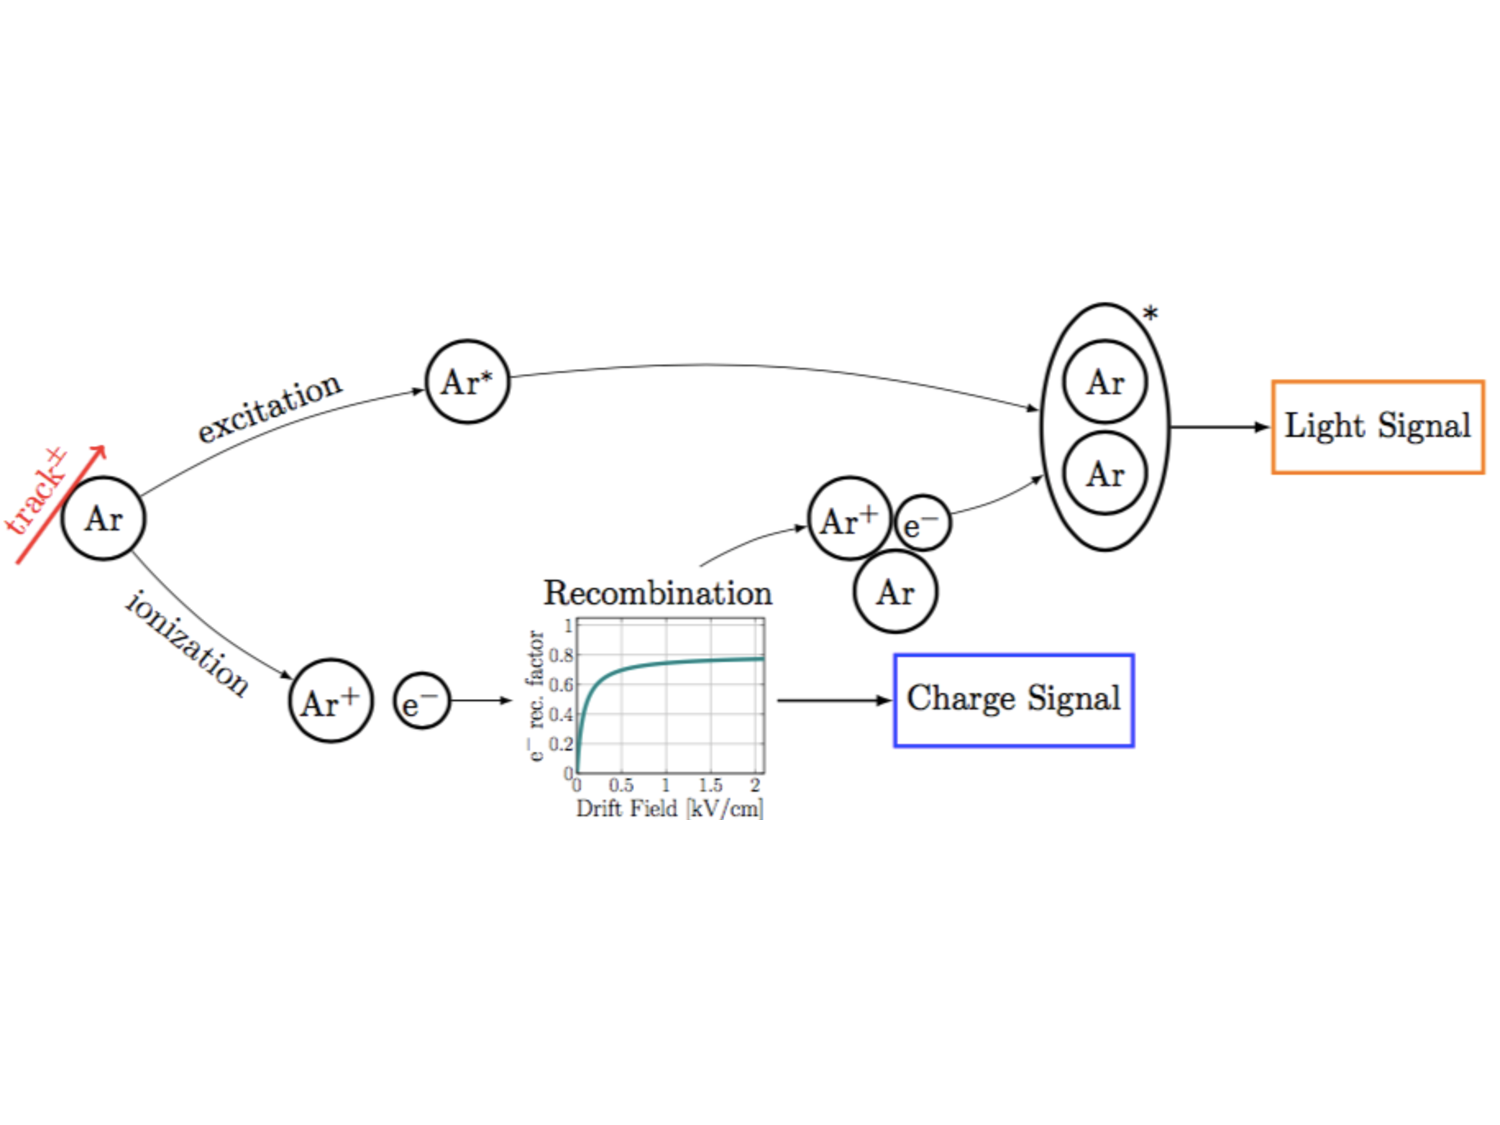
\includegraphics[width=0.95\textwidth]{dppd_6_0}
\end{dunefigure}

The secondary scintillation in the argon gas (i.e., the vapor phase) is unique to the \dword{dpmod} technology. It is the luminescence in gas caused by accelerated electrons in the \efield and in the \dword{lem} anode through Townsend amplification. The S2 signal provides information on the drift time and amount of ionization charge, thus supplementing information from the charge readout on the anode plane. For a given argon gas density, the number of S2 photons is proportional to the number of electrons, the \efield, and the length of the drift path in gas covered by the electrons. In an extraction field of \SI{3.0}{kV/cm} in gas, one electron generates about \num{100} downward-moving photons that cross the \dword{lar} surface \cite{Lux:2018zwd}. The time scale of S2 reflects the extraction time of original ionization from the liquid phase into the gas phase. Therefore, for about \SI{0.5}{kV/cm} drift \efield, this time scale is of the order of hundreds of microseconds. The time between the occurrence of the primary scintillation light and the secondary scintillation light is equivalent to the drift time of the electrons from the ionization coordinate to the \lar surface. This provides an accurate determination of the drift time in the active volume and, hence, a correction tool for the electron attachment (and the associated energy measurement).  

%%%%%%%%%%%%%%%%%%%%%%%%%%%%%%%%%
\subsection{Detector Subsystems and Layout}
\label{sec:dp-pds-overview_layout}

The baseline design of the light collection system calls for \SI{20.3}{cm} (\SI{8}{in}) diameter cryogenic \dwords{pmt} from Hamamatsu Photonics\footnote{Hamamatsu Photonics\texttrademark{}, \url{http://www.hamamatsu.com/resources/pdf/etd/LARGE_AREA_PMT_TPMH1286E.pdf}} (model R5912-MOD20) distributed uniformly on the floor (bottom) of the cryostat and electrically shielded from the bottom cathode plane. Other \dword{pmt} manufacturers being considered include Electron Tubes Limited~\footnote{Electron Tubes Ltd\texttrademark{}, \url{http://www.electron-tubes.co.uk//}} and HZC~\footnote{HZC Photonics\texttrademark{}, \url{http://hzcphotonics.com/en_index.html}.}. According to the baseline design, \dpnumpmtch \dwords{pmt}, approximately \num{1} per \si{m$^2$}, will be installed. The outline of the \dword{dpmod} is shown in Figure~\ref{fig:dppd_3_1}.

\begin{dunefigure}[The \dshort{dpmod} (partly open)]{fig:dppd_3_1}
{The \dword{dpmod} (partly open) with cathode, \dwords{pmt}, \dword{fc}, and anode plane with chimneys.}
%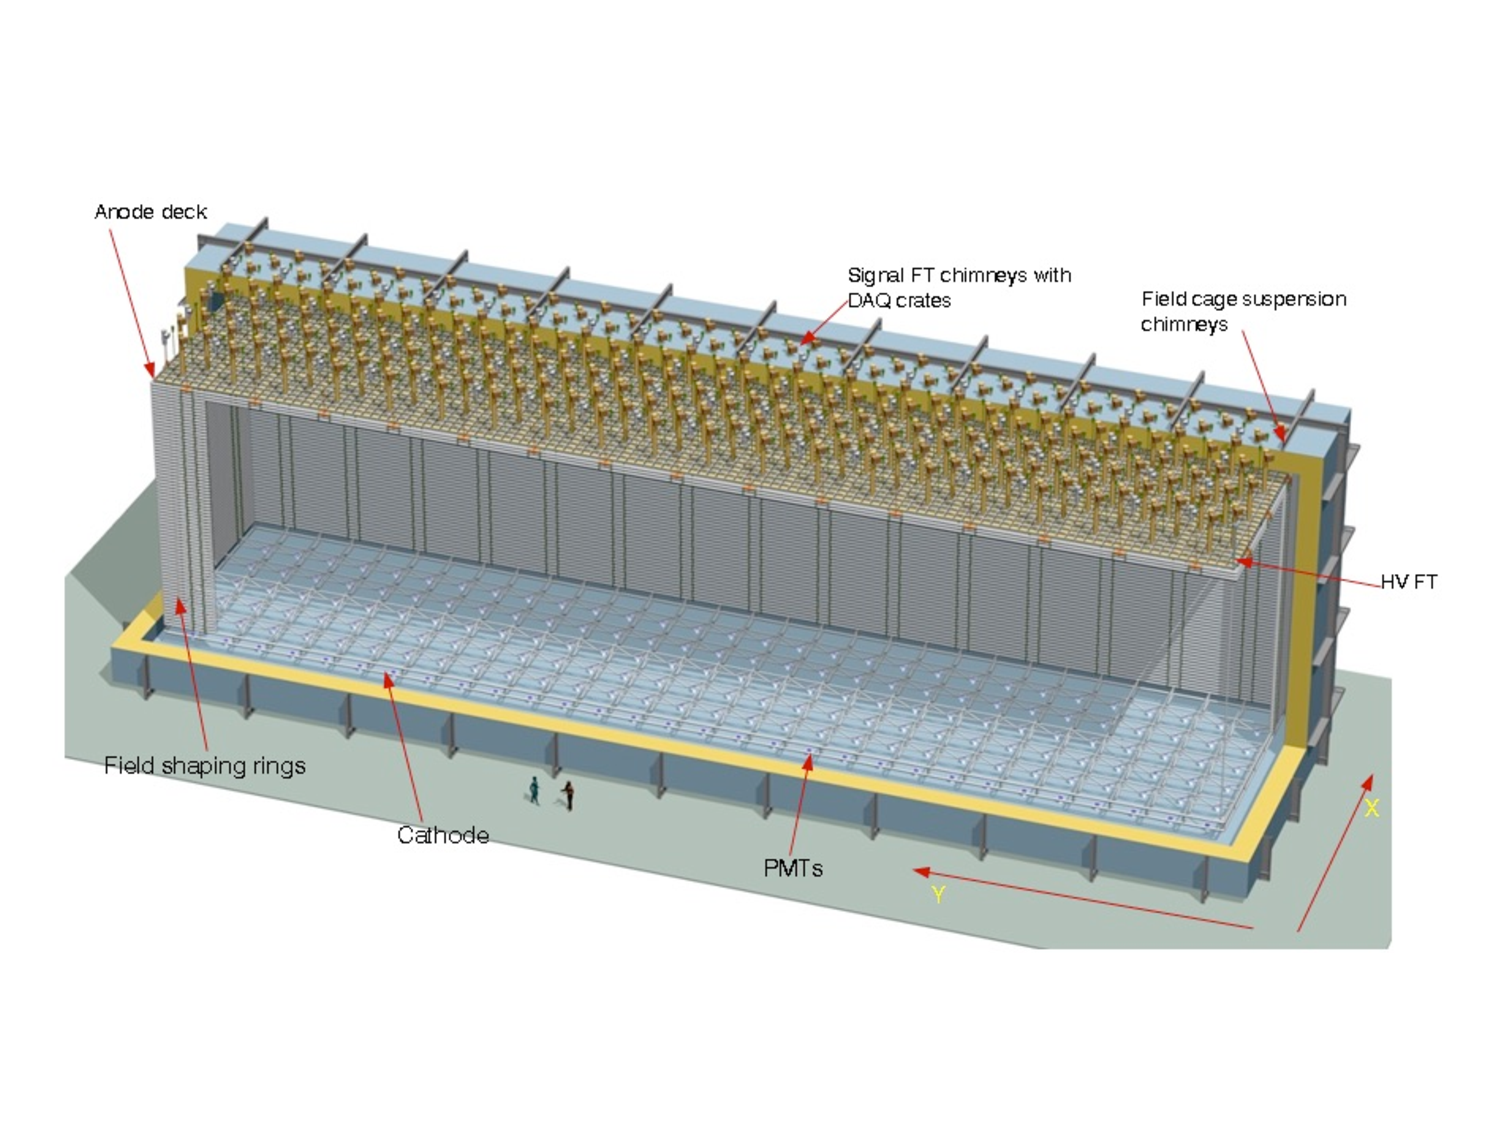
\includegraphics[width=0.95\textwidth]{dppd_3_1}
%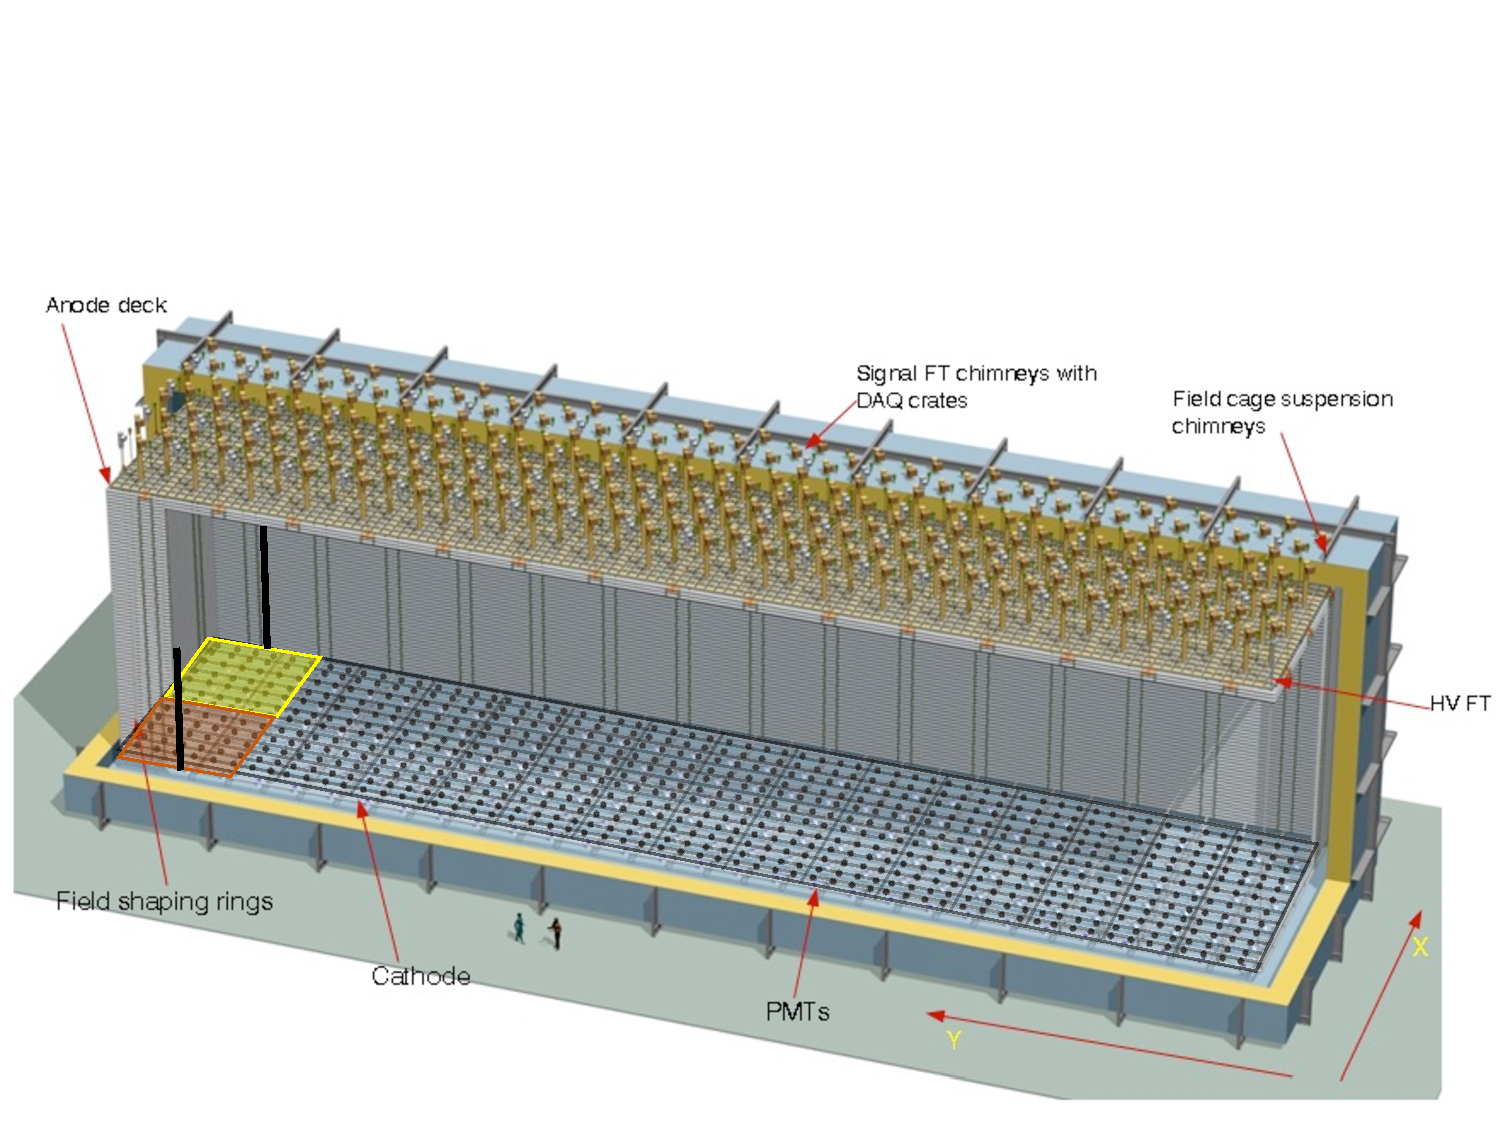
\includegraphics[width=0.95\textwidth]{dppd_1_1_v2}
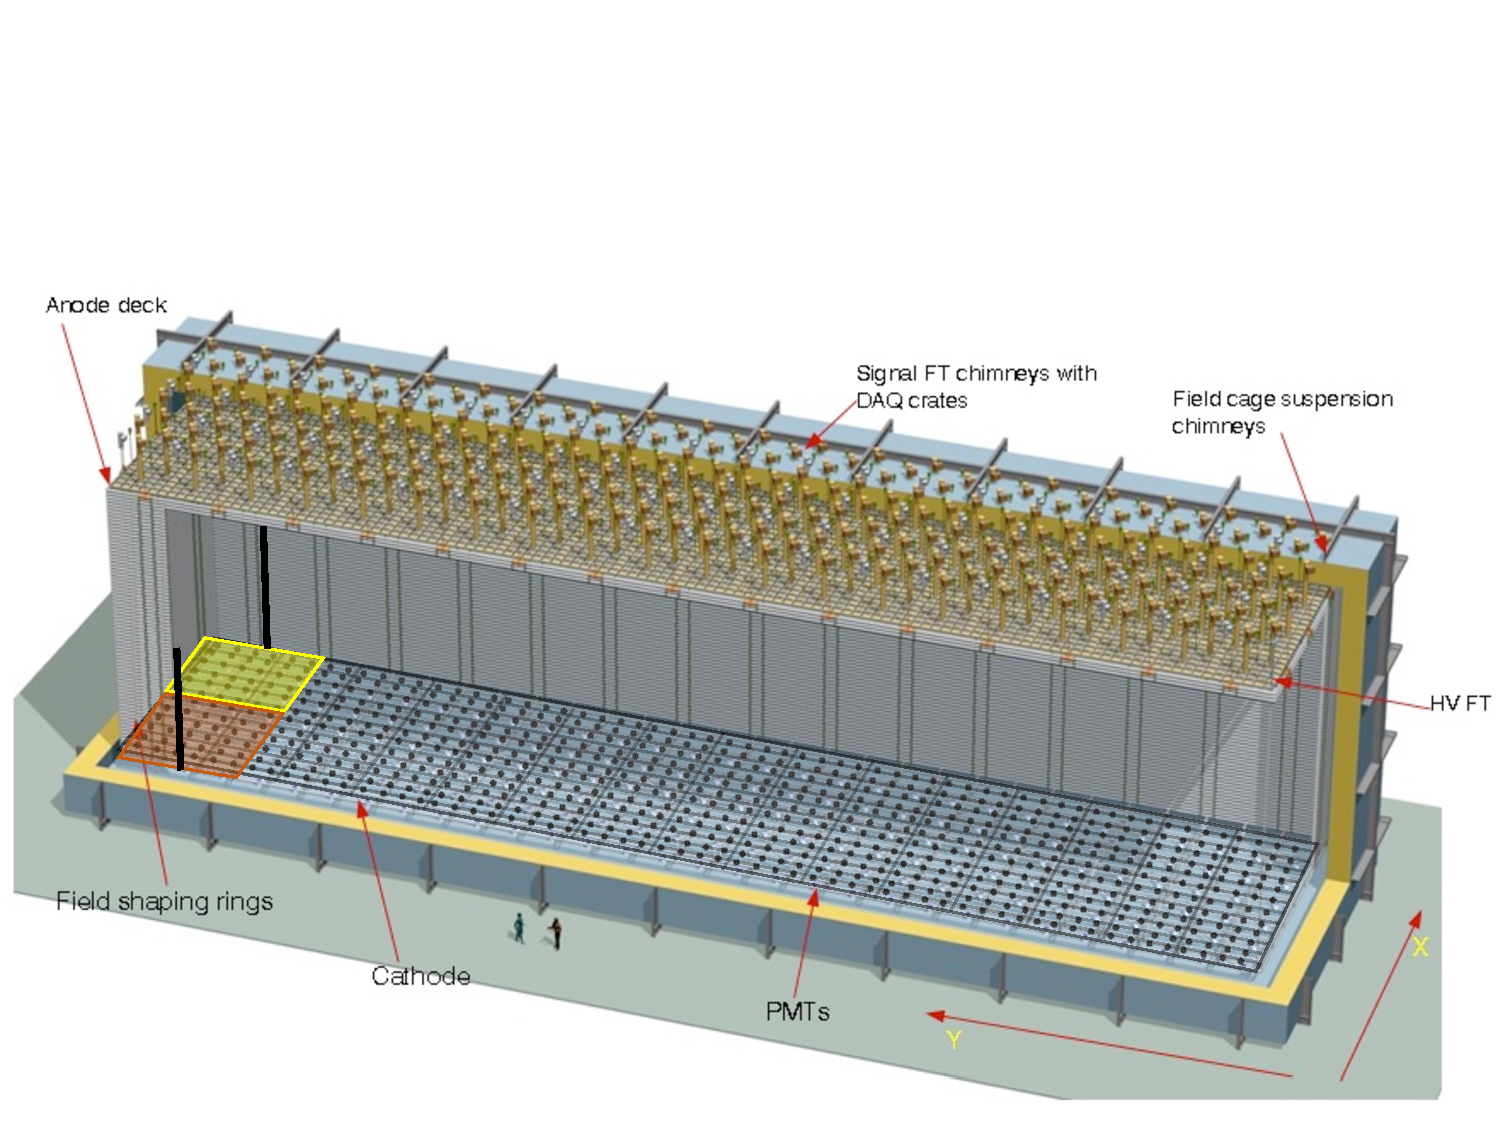
\includegraphics[width=0.95\textwidth]{dppd_1_1_v3}
\end{dunefigure}

The \dwords{pmt} are individually powered to values between \num{1.5} to \num{2.0} \si{\kV} to separately adjust the \dword{pmt} gains. The Hamamatsu R5912 \dwords{pmt} are not sensitive to the \SI{127}{nm} scintillation light, so a wavelength shifter is required. A thin layer of \dword{tpb}~\cite{Francini:2013lua} coating is applied directly on the \dword{pmt} window by evaporation. Section~\ref{sec:dp-pds-photosensors} describes the photosensor system.

The \dpnumpmtch \dwords{pmt} are individually attached to the cryostat floor \SI{1.02}{m} apart in both directions, via a \dword{pmt} support structure that counteracts the \dword{pmt} buoyancy. In order to enhance the light collection and to improve the \dword{pd} response uniformity throughout the entire \dword{tpc} active volume, \dword{tpb} coated reflector/\dword{wls} panels are installed on the top half of the \dword{fc} inner surfaces. Considering the linear relationship between the number of \dwords{pmt} and the detected light yield, and the mild dependence of the \dword{pds} physics performance on light yield and channel granularity, the optimization process that resulted in this baseline design can be considered very robust. The mechanical aspects of the \dword{pmt} support structures and the reflector/\dword{wls} assemblies are described in Section~\ref{sec:dp-pds-mechanics}.

The front-end \dword{pmt} base circuit for reading the \phel signals relies on a positive \dword{hv} supplied to the \dword{pmt} anode and on a grounded photo-cathode. A single cable for each \dword{pmt} carries both power and signal. \dword{hv} and signal splitters located outside the cryostat separate the fast \dword{pmt} response signal from the positive \dword{hv} with capacitive decoupling. The \dword{pds} readout electronics is described in Section~\ref{sec:dp-pds-electronics}.

A photon calibration system is required to determine the \dword{pmt} gain and to monitor the stability of the \dword{pmt} response. The \dword{led}-driven fiber calibration system of the \dword{pds} is described in Section~\ref{sec:dp-pds-calibration}. 

The basic unit of installation/operation is called a sector. The sectors are indicated as transparent red and yellow panels in Figure~\ref{fig:dppd_3_1}. One \dual \dword{pds} sector is \SI{6}{\m} $\times$ \SI{6}{\m} and houses \num{36} \dwords{pmt}. A total of \num{20} sectors are installed in the detector. A single \dword{hv} cable per \dword{pmt} is installed in the cryostat.
The cable trays for the two sectors in Figure~\ref{fig:dppd_3_1} are indicated as black vertical lines.


The \dword{hv} cables penetrate a feedthrough flange and end with SHV connectors, with the calibration fibers also penetrating a feedthrough flange and end with \dword{sma} connectors. One DN250 flange is used per sector of \dual \dword{pds}. One flange houses \num{36} SHV and six \dword{sma} connections. The \dual \dword{pds} design has \num{20} penetrations on the cryostat roof, one per sector. 

The \dword{hv} and signal crates are installed at a density of one per sector for a total of \num{20} \dword{hv}/signal racks on the cryostat roof. Figure~\ref{fig:dppd_1_2} illustrates the layout of the feedthroughs and the \dword{hv}/signal/calibration racks for four sectors. The racks contain the \dword{hv} crates, \dword{hv}/signal splitters, the \dword{utca} crates for the front-end electronics, and the calibration \dword{led} driver and the associated electronics for \num{36} \dwords{pmt}.

\begin{dunefigure}[Cryostat roof layout for \dual \dshort{pds} penetrations]{fig:dppd_1_2}
{The sketch of the cryostat roof layout for \dual \dword{pds} penetrations.}
%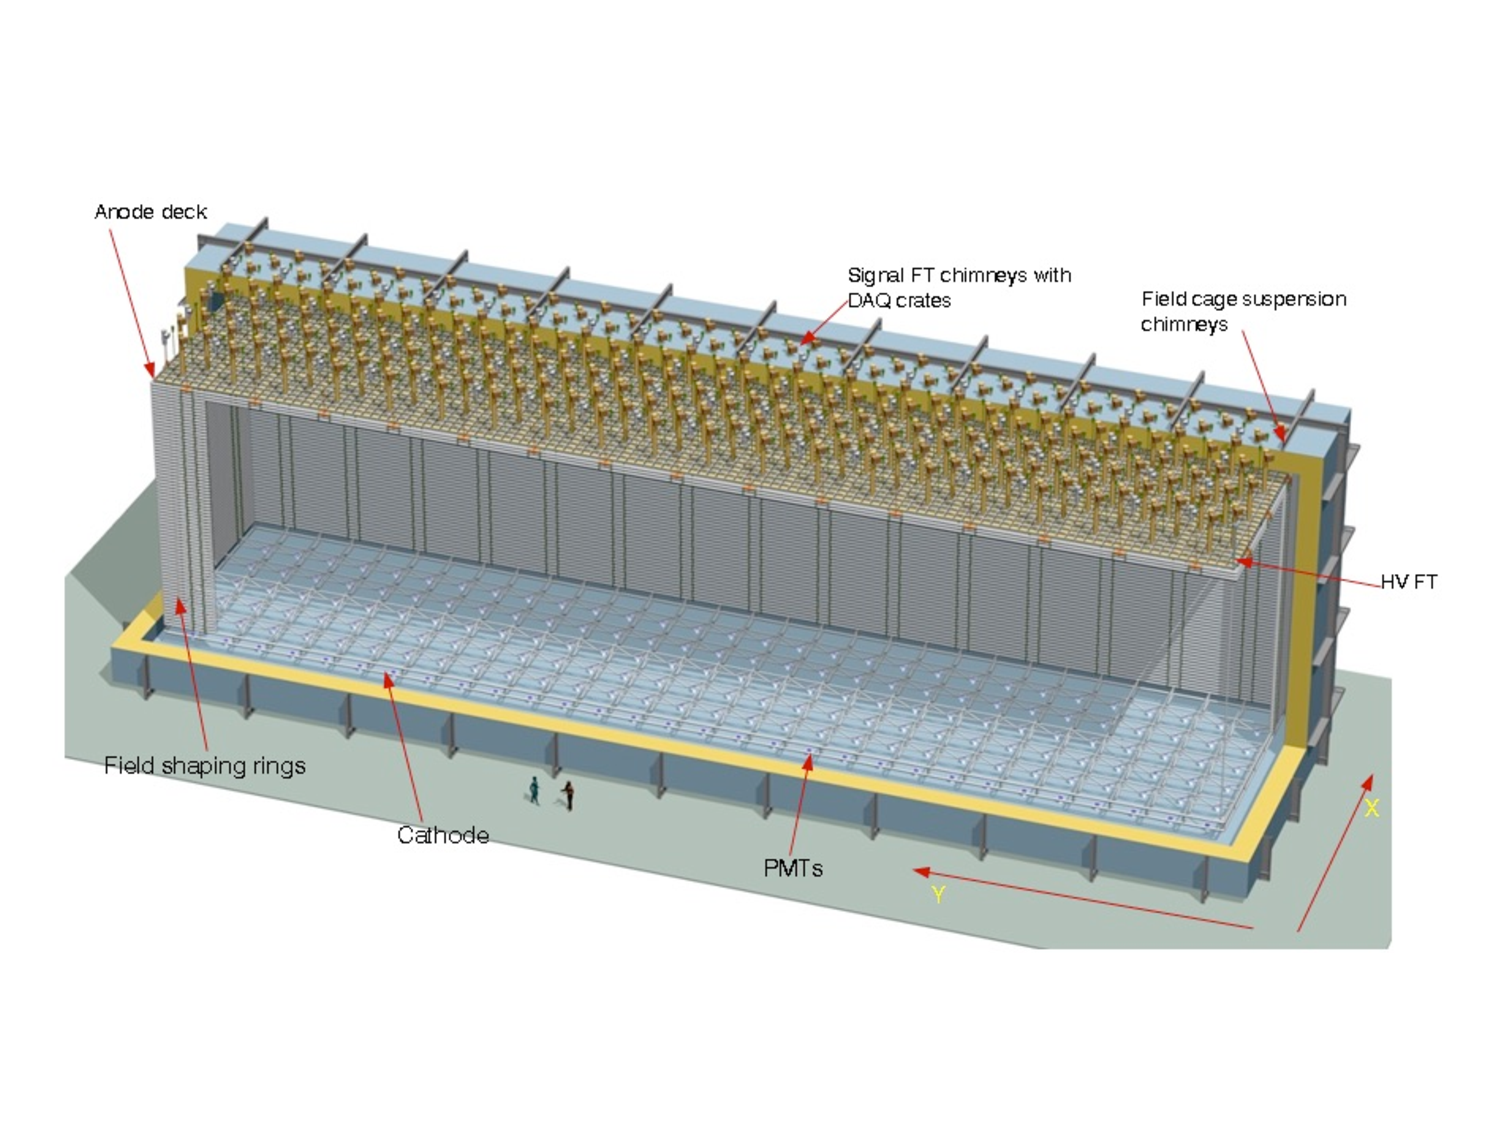
\includegraphics[width=0.95\textwidth]{dppd_3_1}
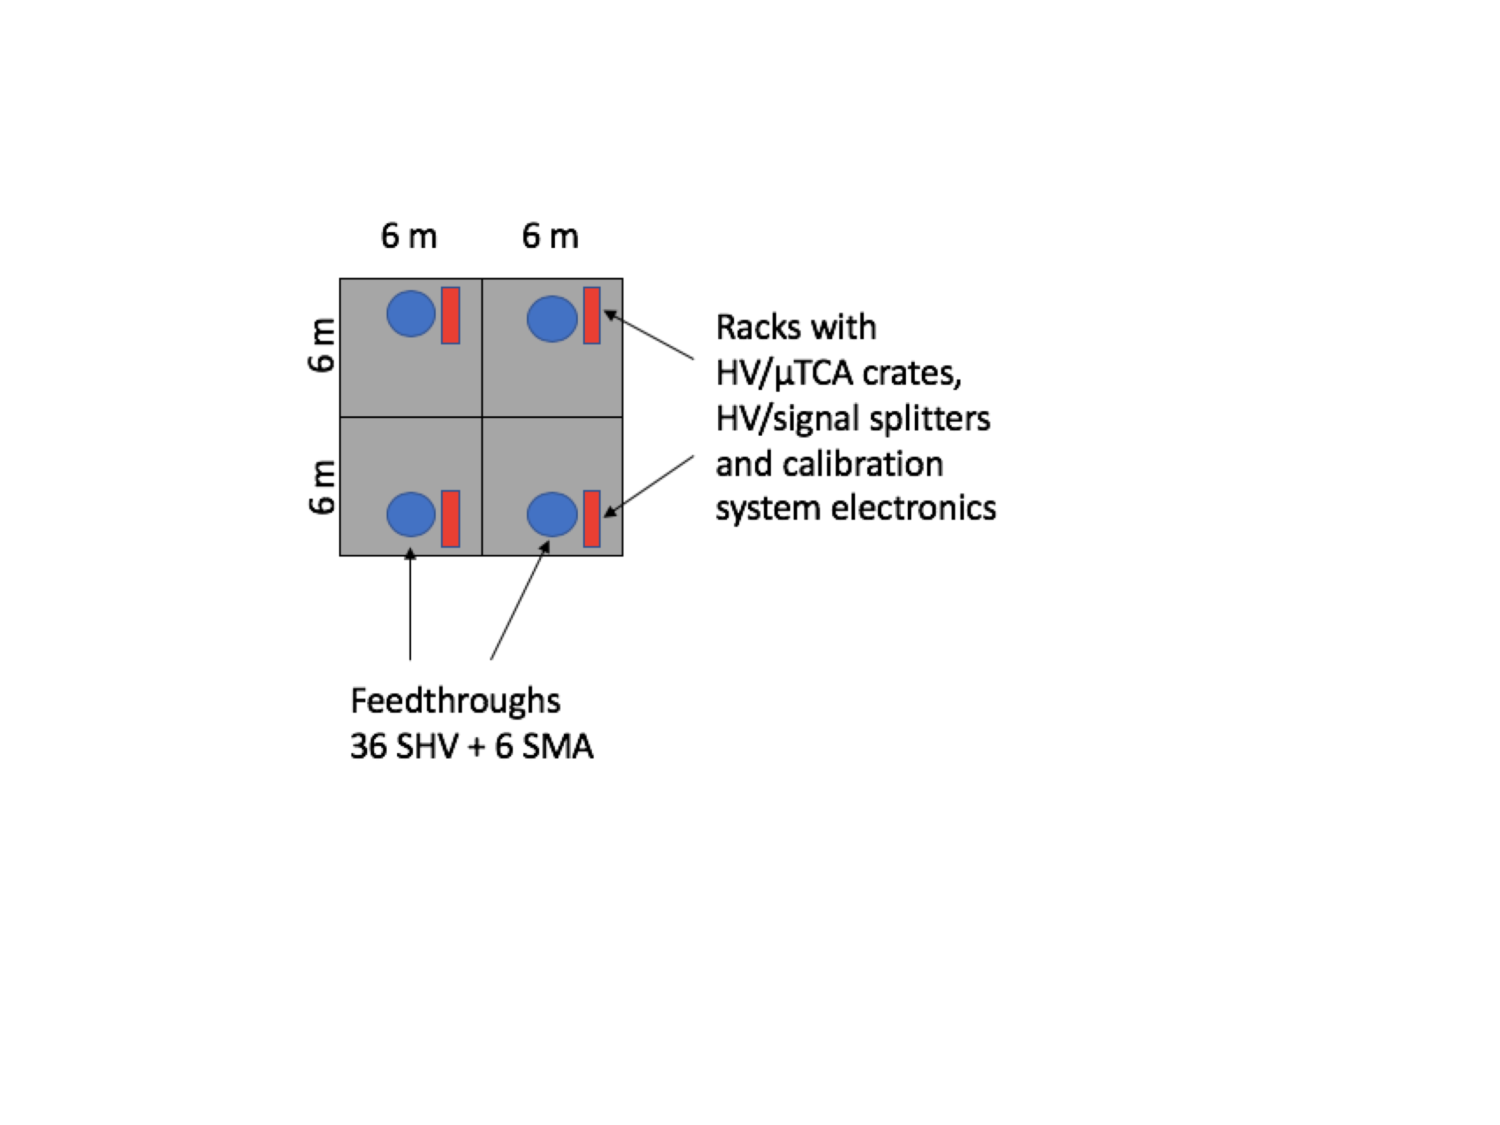
\includegraphics[width=0.55\textwidth]{dppd_1_2}
\end{dunefigure}

The cathode plane, described in Chapter~\ref{ch:dp-hv}, is placed approximately \SI{2}{m} above the bottom of the cryostat. Given the high dielectric constant of the \dword{lar} phase, the \dword{pmt} plane is a safe distance from the cathode plane. To protect the \dwords{pmt}, the \dword{gg} is installed and placed at an identical potential as the \dword{pmt} photocathode (\SI{0}{V}).

%%%%%%%%%%%%%%%%%%%%%%%%%%%%%%%%%
\subsection{Operational Modes} %Principles}
\label{sec:dp-pds-oveerview_operation}

The physics program defines the operational modes of the \dual \dword{pds}. Measuring the neutrino oscillation parameters requires recording events upon receiving an external trigger from the beam, while non-beam physics such as \dwords{snb}, proton decay, or other rare events require special trigger conditions that include the \dword{pds}. Another operation mode is the \Dword{pmt} calibration run, which is initiated by the light calibration system with its dedicated hardware trigger.
%
Thus, the operation modes are
\begin{itemize}
\item external trigger:  
A typical case is when the beam generates a hardware trigger (a beam gate);  it also includes software-generated triggers for test data.
\item non-beam physics trigger: The electronics based on the \dword{pds} signals provides the trigger for, among other events, \dword{snb} and proton decay events;
\item calibration trigger: The trigger is provided by the light calibration system during \dword{pds} calibrations.
\end{itemize}

The external and non-beam physics triggers run in parallel to ensure that rare events like \dwords{snb} are recorded efficiently. 

%%%%%%%%%%%%%%%%%%%%%%%%%%%%%%%%%
\subsection{Detector Design Specifications}
\label{sec:dp-pds-overview_specs}

The \dual \dword{pds} detector specifications are given in Table~\ref{tab:specs:DP-PDS}. The first three rows (DP-FD-3, DP-FD-4, DP-FD-15) give the three \dshort{dpmod} high-level requirements of relevance to the \dword{pds}. The following four requirements (DP-PDS-1, DP-PDS-2, DP-PDS-3, DP-PDS-4) are specific to the \dword{pds}. The physics-driven rationale for each detector specification, and the means to validate them, are also summarized in the table. Validation of the detector specifications uses data from \dword{pds} prototypes (Section~\ref{sec:dp-pds-prototypes}) and from a full simulation and reconstruction of signal and background optical flashes in the \dpmod (Section~\ref{sec:dp-pds-performance}). 

% This file is generated, any edits may be lost.

\begin{longtable}{p{0.14\textwidth}p{0.13\textwidth}p{0.18\textwidth}p{0.22\textwidth}p{0.20\textwidth}}
\caption{Specifications for DP-PDS \fixmehl{ref \texttt{tab:spec:DP-PDS}}} \\
  \rowcolor{dunesky}
       Label & Description  & Specification \newline (Goal) & Rationale & Validation \\  \colhline

   \newtag{SP-FD-1}{ spec:min-drift-field }  & Minimum drift field  &  $>$\,\SI{250}{ V/cm} \newline ( $>\,\SI{500}{ V/cm}$ ) &  Lessens impacts of $e^-$-Ar recombination, $e^-$ lifetime, $e^-$ diffusion and space charge. &  ProtoDUNE \\ \colhline
    
   
  \newtag{SP-FD-2}{ spec:system-noise }  & System noise  &  $<\,\SI{1000}\,e^-$ &  Provides $>$5:1 S/N on induction planes for  pattern recognition and two-track separation. &  ProtoDUNE and simulation \\ \colhline
    
   
  \newtag{SP-FD-3}{ spec:light-yield }  & Light yield  &  $>\,\SI{20}{PE/MeV}$ (avg), $>\,\SI{0.5}{PE/MeV}$ (min) &  Gives PDS energy resolution comparable that of the TPC for 5-7 MeV SN $\nu$s, and allows tagging of $>\,\SI{99}{\%}$ of nucleon decay backgrounds with light at all points in detector. &  Supernova and nucleon decay events in the FD with full simulation and reconstruction. \\ \colhline
    
    \\ \rowcolor{dunesky} \newtag{SP-FD-4}{ spec:time-resolution-pds } & Name: Time resolution \\
    Description & The time resolution of the photon detection system shall be less than 1 microsecond in order to assign a unique event time.   \\  \colhline
    Specification (Goal) &  $<\,\SI{1}{\micro\second}$  ( $<\,\SI{100}{\nano\second}$ ) \\   \colhline
    Rationale &   Enables \SI{1}{mm} position resolution for \SI{10}{MeV} SNB candidate events for instantaneous rate $<\,\SI{1}{m^{-3}ms^{-1}}$.  \\ \colhline
    Validation &   \\
   \colhline

   \newtag{SP-FD-5}{ spec:lar-purity }  & Liquid argon purity  &  $<$\,\SI{100}{ppt} \newline ($<\,\SI{30}{ppt}$) &  Provides $>$5:1 S/N on induction planes for  pattern recognition and two-track separation. &  Purity monitors and cosmic ray tracks \\ \colhline
    

   
  \newtag{DP-PDS-1}{ spec:hit-relative-timing }  & Relative timing accuracy among hits  &  $<\,\SI{100}{ns RMS}$ &  Enable effective clustering of \dword{pmt} signals based on relative hit timing information. &  Full sim/reco of \dword{ndk}, \dword{snb} $\nu$ and radiological events. \\ \colhline
    
   
  \newtag{DP-PDS-2}{ spec:hit-snr }  & Hit signal-to-noise ratio  &  $>\,\num{5}$ &  Efficiently reconstruct single-\phel hits while rate of electronics noise hits remains manageable. &  Single-\phel and baseline noise \dword{rms} measurements in $3\times1\times1$ prototype. \\ \colhline
    
   
  \newtag{DP-PDS-3}{ spec:hit-relative-timing }  & Relative timing accuracy among hits  &  $<\,\SI{100}{ns RMS}$ &  Enable effective clustering of PMT signals based on relative hit timing information. &  Full simulation/reconstruction of NDK, SN $\nu$ and radiological events. \\ \colhline
    
   
  \newtag{DP-PDS-4}{ spec:hit-relative-timing }  & Relative timing accuracy among hits  &  $<\,\SI{100}{ns RMS}$ &  Enable effective clustering of \dword{pmt} signals based on relative hit timing information. &  Full sim/reco of \dword{ndk}, \dword{snb} $\nu$ and radiological events. \\ \colhline
    
   
  \newtag{DP-PDS-5}{ spec:pmt-dark-rate }  & PMT dark count rate  &  $<\,\SI{100}{kHz}$ &  Dark counts should have negligible effect on clustering algorithm and PDS-based calorimetry. &  Characterization of PMTs at cryogenic temperatures prior to installation. \\ \colhline
    
   
  \newtag{DP-PDS-6}{ spec:pds-dynamic-range }  & Dynamic range per channel  &  $>\,\SI{200}{PE}$ &  Avoid hit saturation for energy depositions near cathode plane.  &  Full simulation/reconstruction of beam $\nu$ interactions near cathode plane.  \\ \colhline
    
   \newtag{DP-PDS-7}{ spec:time-resolution-dp-pds }  & Time resolution  &  $<\,\SI{1}{\micro\second}$ \newline ( $<\,\SI{100}{\nano\second}$ ) &  Enables \SI{1}{mm} position resolution for \SI{10}{MeV} SNB candidate events for instantaneous rate $<\,\SI{1}{m^{-3}ms^{-1}}$. &   \\ \colhline
    


\label{tab:specs:DP-PDS}
\end{longtable}
